\documentclass[12pt]{article}
\usepackage[T1]{fontenc}
\usepackage[utf8x]{inputenc}

\usepackage{titling}
\usepackage[top=1in, bottom=1in, left=1in, right=1in]{geometry}
\usepackage{hyperref}
\usepackage{natbib}
\usepackage{graphicx}
\usepackage[table]{xcolor}

\usepackage{caption}
\usepackage{subcaption}






\begin{document}

\begin{titlepage}
	\centering
	
\includegraphics[width=0.15\textwidth]{docs/logo}\par\vspace{1cm}
	{\scshape\LARGE MoSDeF \par}
	\vspace{1cm}
	{\scshape\Large System Requirements Specification\par}
	\vspace{1.5cm}
	{\huge\bfseries General Purpose Molecular Simulation Objects\par}
	\vspace{1cm}
	{\huge\bfseries Version 0.1\par}
	\vspace{2cm}
	{\Large\itshape Co Quach\par}
	{\Large\itshape Justin Gilmer\par}
	{\Large\itshape Parashara Shamaprasad\par}
	{\Large\itshape Ray Matsumoto\par}
	{\Large\itshape Umesh Timalsina\par}

	\vfill

% Bottom of the page
	{\large \today\par}
\end{titlepage}

{\centering \section*{Overview}}
\noindent The General Purpose Molecular Simulation Objects (\textbf{GPMSO}) will be a comprehensive representation of data types, capabilities and structural representation of objects needed to efficiently represent chemical topology/system which can be leveraged to write out files necessary for different simulation engines as well as cover heterogeneous domains of molecular simulations. \\~\\
The objectives of this \textbf{GPMSO} are:
\begin{enumerate}
    \item Have an efficient in--memory representation of different aspects of a chemical topology like \texttt{Sites}, \texttt{Connections}, \texttt{Potentials}, \texttt{ForceFields} etc...
    \item Have an efficient serialized/disk representation of the system which can be loaded to create an object and vice versa.
    \item Have a convenient interface for extension/interfacing with other specifications in this realm.
    \item Have support for mathematical expressions and parameters that would be used to represent different physical quantities, preferably with support for different unit systems.
\end{enumerate}

To that end, this document serves as a starting point for developers/software scientists looking for standard practices and avoiding pitfalls in designing/implementing a molecular simulation objects.

{\centering \section*{Revision History}}
\begin{table}[ht]
    \centering
    \begin{tabular}{|c|c|c|c|}
    \hline
    \textbf{Date} &  \textbf{Version} & \textbf{Description}  & \textbf{Link} \\
    \hline
    \today & 0.1 & Initial Draft & click to follow \\
    \hline
    \end{tabular}
\end{table}

\pagebreak
\tableofcontents
\thispagestyle{empty}
\pagebreak


% Major Sections
\section{Introduction}
System requirements specification (\textbf{SRS}) for the General Purpose Molecular Simulation Objects (\textit{GPMSO}) is introduced in this section.

\subsection{Specification Definition}
This specification documents the system--level requirements for \textit{GPMSO}.

\subsection{Specification Objectives}
The objectives of this specification are:

\begin{itemize}
    \item Provide a system overview of the \textit{GPMSO} including definitions, goals, objectives, context and major capabilities.
    \item To formally specify its associated:
      \begin{itemize}
          \item Functional requirements via capabilities
          \item Data requirements via constituents and properties
      \end{itemize}
\end{itemize}

\subsection{Intended Audiences}
The intended audiences for this document are:

\begin{enumerate}
    \item Software developers/Research Scientists/Engineers looking for high level overview of a molecular simulation object
    \item Researchers using different simulation engines for their molecular simulation
\end{enumerate}
eterized System Representat
\subsection{Specification Overview}
% ToDO: Write this after Functional requirements
This document is organized as follows:
\begin{itemize}
    \item \textbf{Introduction}: Provides an introduction to this specification
    \item \textbf{GPMSO System Overview}: Elaborates the specification concepts
    \item \textbf{Next Steps}: Provides an overview of the plan on further refining this document
\end{itemize}

\pagebreak
\section{GPMSO System Overview}
Any general purpose representation of a molecular system that could be leveraged for molecular simulation purposes has following advantages:
\begin{enumerate}
    \item Support for multiple different chemistries allows for research groups/ labs not to rely on in house tools but rather harness the power of open--source development practices to solve in--house research problems
    \item Single avenue for maintenance and extension
    \item Possibility of a well maintained, documented open--source code base supporting the needs of a plethora of researchers/software developers working in the area with quick bug--fixes and scheduled releases
\end{enumerate}

\noindent To specify a typed system specification we need the following containers:

\begin{enumerate}
    \item The base container (\texttt{System}): A container object representing physical constructs as well as the necessary physics that define a molecular system

    \item The non-physical interaction container (\texttt{PotentialCollection}): A container representing non-physical constructs like energies, functional forms of interactions etc… in a typed/parameterized molecular system
\end{enumerate}

We should be able to create a \texttt{PotentialCollection} from a parameterized/ typed \texttt{System} container. The constituents, properties and capabilities of these containers are described in Section~\ref{def:Topology} and Section~\ref{def:ForceField}.

\subsection{System}
\label{def:Topology}
As mentioned earlier, a \texttt{System} is a collection of physical constructs that define a molecular system. The constructs (constituents, properties and capabilities) to define a parameterized \texttt{System} are shown in  Table~\ref{tab:TopologySpec}:

 \rowcolors{2}{gray!35}{white}
\begin{table}[ht]
    \centering
     \caption{Parameterized \texttt{System} representation}
    \begin{tabular}{|l|}
         \hline
         \rowcolor{gray!50}
        \texttt{System}  \\
         \hline
         \textbf{Constituents} \\
         \texttt{Site} (0..*) \\
         \texttt{Connection} (0..*)\\
         \texttt{Potential} (0..*)\\
         \hline
         \textbf{Properties}\\
         \texttt{Metadata} \\
         \hline
         \textbf{Capabilities}\\
         \hline
         - Easy lookup for constituents \\
         - Positions lookup \\
         - Identifiable connections \\
         - Easy bookkeeping for potentials/functional forms \\
         - Formal serialized representation (deterministic schema) \\
         - Visualization \\
         - Support for different file formats (dependent on the simulation engine) \\
         - Interaction/Composition with other \texttt{Systems}\\
         - Constituent datatype validation \\
         - Unit support \\
         - Extensible architecture \\
         - Easy conversion to/and from other similar \texttt{System} objects\\
         - Track changes \\

        \hline

    \end{tabular}
    \label{tab:TopologySpec}
\end{table}

\subsubsection{Constituents}
A \texttt{System} container should have following constituents:
\begin{itemize}
    \item \texttt{Site}: \texttt{Site} represents any general interaction site in a molecular simulation. There can be any number of \texttt{Site} and their variants in a \texttt{System} container.

    \item \texttt{Connection}: A \texttt{Connection} stores data about connections between sites. There can be any number of \texttt{Connection} and its variants in a \texttt{System} container.

    \item \texttt{Potential}: \texttt{Potential} stores a general interaction between components of a chemical topology that can be specified by a mathematical expression and parameters. \texttt{Potentials} are generally associated with a typed/parameterized \texttt{System} container and there can be any number of \texttt{Potential} and its variants in it.
\end{itemize}

\subsubsection{Properties}
Generally, the following properties should be associated with a \texttt{System} container:

\begin{itemize}
    \item \texttt{Metadata}: Metadata regarding combining rules, units, parametric solvers etc...
\end{itemize}

\subsubsection{Capabilities}
As shown in Table~\ref{tab:TopologySpec}, a \texttt{System} should be able easily lookup its constituents based on identifiable boundaries like residues or chains, shared attributes of its constituents like all sites of a particular type, all potentials of a particular type and many other constructs that might be relevant to molecular simulation. Lookup for constituents should facilitate conversion to other standard representation as well writers that generate files for different simulation engines. A \texttt{System} container should be able to locate every constituent \texttt{Site} within in 3D-Euclidean space and alter their positions. A \texttt{System} should also be able to track changes on its constituents.

Additionally, a \texttt{System} container should also have a deterministic schema for its serialized representation such that a seamless conversion from disk--to--memory or memory--to--disk is possible. A \texttt{System} container should also have support for different file formats that are required by a diverse array of simulation engines and there should be relatively painless way of handling file--format support.

Moreover, a \texttt{System} container should be able to support a \texttt{Graph} representation and thus associated visualization techniques.

Additionally, a \texttt{System} container should be capable of validating constituent data types and provide support for representing physical quantities in different unit systems with preferred defaults.

Furthermore, we should be able to get a \texttt{PotentialCollection} container from a \texttt{System} representation.

Finally, the architecture of the \texttt{System} container should be built in such a way that its easily extensible and can be composed with other containers having the same specification.

\subsection{PotentialCollection}
\label{def:ForceField}
As mentioned earlier, a \texttt{PotentialCollection} is a non--physical interaction container containing different \texttt{Potential} constituents.  The constructs (constituents, properties and capabilities) to define a \texttt{PotentialCollection} are shown in  Table~\ref{tab:ForceFieldSpec}.


 \rowcolors{2}{gray!35}{white}
\begin{table}[ht]
    \centering
     \caption{\texttt{PotentialCollection} representation}
    \begin{tabular}{|l|}
         \hline
         \rowcolor{gray!50}
         \texttt{PotentialCollection}  \\
         \hline
         \textbf{Constituents} \\
         \texttt{Potential} (0..*)\\
         \hline
         \textbf{Properties}\\
         \texttt{Metadata} \\
         \hline
         \textbf{Capabilities}\\
         \hline
         - Capture existing standard forcefields in a meaningful way\\
         - Easy lookup for constituents\\
         - Identifiable relationships between different Potentials\\
         - Formal serialized representation \\
         - Standard human readable formats like XML/JSON \\
         - Unit support\\
         - Constituent datatype validation\\
         - Extensible architecture\\
         - Track changes\\
         - Provenance \\
        \hline
    \end{tabular}
    \label{tab:ForceFieldSpec}
\end{table}

\subsubsection{Constituents}
\begin{itemize}
    \item \texttt{Potential}: \texttt{Potential} stores a general interaction between components of a chemical topology that can be specified by a mathematical expression and parameters. A \texttt{PotentialCollection} container can contain any number of \texttt{Potential} and its variants in it. The \texttt{PotentialCollection}'s \texttt{Potentials} can be used to provide \texttt{Potential} information for the \texttt{System}'s constituent sites and connections.
\end{itemize}

\subsubsection{Properties}
\begin{itemize}
    \item \texttt{Metadata}: Information like \texttt{name}, \texttt{version}, \texttt{nonBonded14Scale}, \texttt{electrostatics14Scale} etc...  should be considered as Metadata property for the \texttt{PotentialCollection} representation.
\end{itemize}

\subsubsection{Capabilities}
As shown in Table~\ref{tab:ForceFieldSpec}, a  \texttt{PotentialCollection} should have easy lookup for its constituents based on shared attributes of its constituents like all \texttt{Potentials} of a particular type, shared association etc... A \texttt{PotentialCollection} container should also be able to track changes of its constituents.

Additionally, A \texttt{PotentialCollection} container should also have a deterministic schema for  its  serialized  representation  such  that  a  seamless  conversion  from  disk–to–memory  or memory–to–disk is possible. While there can be many ways to have a standard serialized representation, any such representation should be able to:

\begin{enumerate}
    \item Be represented in a human readable textual format like XML/JSON
    \item Capture necessary information from the existing standard forcefields used in molecular simulations
\end{enumerate}

Additionally, a \texttt{PotentialCollection} container should be capable of validating constituent data types and provide support for representing physical quantities in different unit systems with preferred defaults.

Finally, the architecture of \texttt{PotentialCollection} should be built in such away that its easily extensible and can be composed with other containers having the same specification.

\subsection{Constituents}
This section describes the constituent members of the containers described in Sections~\ref{def:Topology} and \ref{def:ForceField}.

\subsubsection{Site}
\texttt{Site} represents any general interaction site in a molecular simulation. \texttt{Site} should be specified to be as general as possible, making no assumptions about representing atoms or beads, or having mass or charge. That is, a \texttt{Site} can represent an atom in an atomistic system, a bead in a coarse-grained system, and much more. A common abstraction for \texttt{Site} should be developed from gleaning common properties that different variants of a \texttt{Site} share.

Table~\ref{tab:SiteSpec} shows  the constructs (associations, properties and capabilities) to define a \texttt{Site}.

 \rowcolors{2}{gray!35}{white}
\begin{table}[ht]
    \centering
     \caption{\texttt{Site} representation}
    \begin{tabular}{|l|}
         \hline
         \rowcolor{gray!50}
         \texttt{Site}  \\
         \hline
         \textbf{Associations} \\
         \hline
         \texttt{--> Potential}\\
         \textbf{Properties}\\
         \hline
         \texttt{name} \\
         \texttt{labels} \\
         \texttt{position}\\
         \texttt{Metadata}\\
         \hline
         \textbf{Capabilities}\\
         \hline
         - Datatype validation \\
         - Standard serialized representation \\
         - Easy look up for associated \texttt{Potential} \\
         - Unit support \\
        \hline
    \end{tabular}
    \label{tab:SiteSpec}
\end{table}
\paragraph{Associations}
A directed one--to--one association from a  \texttt{Site} to its associated \texttt{Potential} can/should exist.
\paragraph{Properties}
\begin{itemize}
    \item \texttt{name}: Identifier name of the \texttt{Site}
    \item \texttt{labels}: Labels to add the \texttt{Site} to a group of \texttt{Sites}
    \item \texttt{position}: The 3D--Cartesian coordinates of the \texttt{Site} when in the \texttt{System}
    \item \texttt{Metadata}: Miscellaneous properties of the \texttt{Site}
\end{itemize}
\paragraph{Capabilities}
Any \texttt{Site} and its variant should be capable of validating constituent data types and provide support for representing physical quantities in different unit systems with preferred defaults. With the requirement that \texttt{System} container in which the \texttt{Site} resides should support on disk serialization, a \texttt{Site} should have a standard serialized representation as well. Additionally, a \texttt{Site} should facilitate easy lookup for its associated \texttt{Potential} (if it exists).

\paragraph{Example Variants} Some variants (non-exhaustive) of \texttt{Site} are shown in Table~\ref{tab:ExampleSites}.

 \rowcolors{2}{gray!35}{white}
\begin{table}[ht]
    \centering
    \caption{Example variants of \texttt{Site}}
    \label{tab:ExampleSites}
    \begin{subtable}[h]{0.45\textwidth}
    \caption{\texttt{Atom}}
    \begin{tabular}{|l|}
         \hline
         \rowcolor{gray!50}
         \texttt{Atom}  \\
         \hline
         \textbf{Associations} \\
         \hline
         \texttt{--> AtomType}\\
         \textbf{Properties}\\
         \hline
         \texttt{charge} \\
         \texttt{mass} \\
         \texttt{element}\\
         \texttt{...}\\
         \hline
         \textbf{Capabilities}\\
         \hline
         - Associate with an \texttt{AtomType} (\texttt{Potential})\\
         - A \texttt{Bond} (\texttt{Connection}) can associate\\
        \hline
    \end{tabular}
    \end{subtable}
    \hfill
    \begin{subtable}[h]{0.45\textwidth}
    \caption{\texttt{Bead}}
    \begin{tabular}{|l|}

         \hline
         \rowcolor{gray!50}
         \texttt{Bead}  \\
         \hline
         \textbf{Associations} \\
         \hline
         \texttt{--> AtomType}\\
         \textbf{Properties}\\
         \hline
         \texttt{charge} \\
         \texttt{mass} \\
         \texttt{...}\\
         \texttt{...}\\
         \hline
         \textbf{Capabilities}\\
         \hline
        - Associate with an \texttt{AtomType} (\texttt{Potential})\\
        - A \texttt{Bond} (\texttt{Connection}) can associate\\
        \hline
    \end{tabular}
    \end{subtable}
    \newline
    \vspace*{1 cm}
    \newline
    \begin{subtable}[h]{0.45\textwidth}
    \caption{\texttt{VirtualSite}}
    \begin{tabular}{|l|}

         \hline
         \rowcolor{gray!50}
         \texttt{VirtualSite}  \\
         \hline
         \textbf{Associations} \\
         \hline
         \texttt{--> AtomType}\\
         \textbf{Properties}\\
         \hline
         \texttt{charge} \\
         \texttt{mass} \\
         \texttt{position}\\
         \texttt{...}\\
         \hline
         \textbf{Capabilities}\\
         \hline
         - A \texttt{Bond} (\texttt{Connection}) can associate\\
         - ..\\
        \hline
    \end{tabular}
    \end{subtable}

\end{table}


\pagebreak


\subsubsection{Connection}
A \texttt{Connection} stores data about connections between sites. Any connected groups (\texttt{Bonds}, \texttt{Angles}, \texttt{Dihedrals}, etc...) should be abstracted as a \texttt{Connection}. A common abstraction for \texttt{Connection} should be developed from gleaning common properties that different variants of a \texttt{Connection} share.

Table~\ref{tab:ConnSpec} shows  the constructs (associations, properties and capabilities) to define a \texttt{Connection}.

\rowcolors{2}{gray!35}{white}
\begin{table}[ht]
    \centering
     \caption{\texttt{Connection} representation}
    \begin{tabular}{|l|}
         \hline
         \rowcolor{gray!50}
         \texttt{Connection}  \\
         \hline
         \textbf{Associations} \\
         \hline
         \texttt{--> Potential}\\
         \texttt{--> Site (0..n)}\\
         \textbf{Properties}\\
         \hline
         \texttt{name} \\
         \texttt{Metadata}\\
         \hline
         \textbf{Capabilities}\\
         \hline
         - Datatype validation \\
         - Standard serialized representation \\
         - Easy look up for associated \texttt{Potential} \\
         - Unit support \\
         - Members query \\
         - Duplication capabilities \\
        \hline
    \end{tabular}
    \label{tab:ConnSpec}
\end{table}

\paragraph{Associations}
\begin{itemize}
    \item A directed one–to–one association from a \texttt{Connection} to its associated \texttt{Potential} can/should exist.
    \item A directed one--to--many association from a \texttt{Connection} to its member \texttt{Sites} must exist.
\end{itemize}
\paragraph{Properties}
\begin{itemize}
    \item \texttt{name}: Identifier name of the \texttt{Site}
    \item \texttt{Metadata}: Miscellaneous properties of the \texttt{Connection}
\end{itemize}
\paragraph{Capabilities}
Any \texttt{Connection} and its variant should be capable of validating constituent data types and provide support for representing physical quantities in different unit systems with preferred defaults. With the requirement that \texttt{System} container in which the \texttt{Connection} resides should support on disk serialization, a \texttt{Connection} should have a standard serialized representation as well. A \texttt{Connection} should be also able to query its associated members.

\paragraph{Example Variants}  Some variants (non-exhaustive) of \texttt{Connection} are shown in Table~\ref{tab:ExampleConnections}.

\rowcolors{2}{gray!35}{white}
\begin{table}[ht]
    \centering
    \caption{Example variants of \texttt{Connection}}
    \label{tab:ExampleConnections}
    \begin{subtable}[h]{0.45\textwidth}
    \caption{\texttt{Bond}}
    \begin{tabular}{|l|}
         \hline
         \rowcolor{gray!50}
         \texttt{Bond}  \\
         \hline
         \textbf{Associations} \\
         \hline
         \texttt{--> BondType}\\
          \texttt{--> Atom (2..2)}\\

         \textbf{Properties}\\
         \hline
            ...\\
         \texttt{...}\\
         \hline
         \textbf{Capabilities}\\
         \hline
         - Associate with a \texttt{BondType} (\texttt{Potential})\\
         - Associate with an \texttt{Atom} (\texttt{Site})\\
        \hline
    \end{tabular}
    \end{subtable}
    \hfill
    \begin{subtable}[h]{0.45\textwidth}
       \caption{\texttt{Angle}}
    \begin{tabular}{|l|}
         \hline
         \rowcolor{gray!50}
         \texttt{Angle}  \\
         \hline
         \textbf{Associations} \\
         \hline
         \texttt{--> AngleType}\\
          \texttt{--> Atom (3..3)}\\

         \textbf{Properties}\\
         \hline
            ...\\
         \texttt{...}\\
         \hline
         \textbf{Capabilities}\\
         \hline
         - Associate with a \texttt{BondType} (\texttt{Potential})\\
         - Associate with an \texttt{Atom} (\texttt{Site})\\
        \hline
    \end{tabular}
    \end{subtable}
    \newline
    \vspace*{1 cm}
    \newline
    \begin{subtable}[h]{0.45\textwidth}
    \caption{\texttt{Improper}}
    \begin{tabular}{|l|}

         \hline
         \rowcolor{gray!50}
         \texttt{Improper}  \\
         \hline
         \textbf{Associations} \\
         \hline
         \texttt{--> ImproperType}\\
         \texttt{--> Atom (3..3)}\\
         \textbf{Properties}\\
         \hline
            ...\\
             \texttt{...}\\
         \hline
         \textbf{Capabilities}\\
         \hline
         - Associate with an \texttt{ImproperType} (\texttt{Potential})\\
        \hline
    \end{tabular}
    \end{subtable}

\end{table}

\pagebreak

\subsubsection{Potential}
\texttt{Potential} stores a general interaction between components of a chemical system that can be specified by a mathematical expression. The functional form of the potential together with the associated parameters should be stored in an efficient way by the \texttt{Potential}. \texttt{Potential} is agnostic to the instantiation of the potential, which can be e.g. a non-bonded potential, a bonded potential, an angle potential, a dihedral potential, etc...

Table~\ref{tab:PotSpec} shows  the constructs (associations, properties and capabilities) to define a \texttt{Potential}.

\rowcolors{2}{gray!35}{white}
\begin{table}[ht]
    \centering
     \caption{\texttt{Potential} representation}
    \begin{tabular}{|l|}
         \hline
         \rowcolor{gray!50}
         \texttt{Potential}  \\
         \hline
         \textbf{Properties}\\
         \hline
         \texttt{name} \\
         \texttt{expression} \\
         \texttt{independent\_variables}\\
         \texttt{Metadata}\\
         \hline
         \textbf{Capabilities}\\
         \hline
         - Datatype validation \\
         - Standard serialized representation \\
         - Unit support \\
         - Chemical grammar support \\
        \hline
    \end{tabular}
    \label{tab:PotSpec}
\end{table}

\paragraph{Associations}
\begin{itemize}
    \item A \texttt{Potential} doesn't have any association.
\end{itemize}
\paragraph{Properties}
\begin{itemize}
    \item \texttt{name}: Identifier name of the \texttt{Potential}
    \item \texttt{Potential}: Miscellaneous properties of the \texttt{Potential}
\end{itemize}
\paragraph{Capabilities}
Any \texttt{Potential} and its variant should be capable of validating constituent data types and provide support for representing physical quantities in different unit systems with preferred defaults. The data type validation capabilities include monitoring its mathematical expression along with their parameters, which may be available for some of the Variants.

With the requirement that \texttt{System} container in which the \texttt{Potential} resides should support on disk serialization, a \texttt{Potential} should have a standard serialized representation as well.

\paragraph{Example Variants}  Some variants (non-exhaustive) of \texttt{Potential} are shown in Table~\ref{tab:ExamplePotentials}.


\rowcolors{2}{gray!35}{white}
\begin{table}[ht]
    \centering
    \caption{Example variants of \texttt{Potential}}
    \label{tab:ExampleConnections}
    \begin{subtable}[h]{0.45\textwidth}
    \centering
    \caption{\texttt{BondType}}

    \begin{tabular}{|l|}
         \hline
         \rowcolor{gray!50}
         \texttt{BondType}  \\
         \hline
         \textbf{Properties}\\
         \hline
         parameters\\
         \texttt{...}\\
         \hline
         \textbf{Capabilities}\\
         \hline
         - Avoid Duplication \\

        \hline
    \end{tabular}
    \end{subtable}
    \hfill
    \begin{subtable}[h]{0.45\textwidth}
       \caption{\texttt{ParametricPotential}}
       \centering
    \begin{tabular}{|l|}
         \hline
         \rowcolor{gray!50}
         \texttt{ParametricPotential}  \\
         \hline

         \textbf{Properties}\\
         \hline
            ...\\
         \texttt{...}\\
         \hline
         \textbf{Capabilities}\\
         \hline
         - Parametrize\\
        \hline
    \end{tabular}
    \end{subtable}
\end{table}


\pagebreak
\subsection{System Representation Diagrams}
The overall block diagram of the \texttt{System} container can be represented via webgme metamodel as shown in Figure~\ref{fig:TopoDiagram}. In the diagram, the black lines with diamond endings show a containment relationship and the associated cardinality of the containment. The blue lines show a pointer or one--to--one association. The red lines show inheritance and pink lines show a set or one--to--many association. Some identifiable attributes for some of the classes are shown in the figure as well. Additionally, the nodes with gray colored titles are meant to be abstract.

As shown in Figure~\ref{fig:TopoDiagram}, a \texttt{System} can contain any number of \texttt{Site}. \texttt{Atom}, \texttt{Bead} and \texttt{GenericSite} inherit from \texttt{Site}. A \texttt{Bond} has \texttt{src} and \texttt{dst} pointers that have to be an \texttt{Atom}. Similarly, a the set \texttt{connectionMembers} that contains fixed number of \texttt{Atoms}(predefined cardinality) is associated with each \texttt{Connection}.

\begin{figure}[ht]
    \centering
    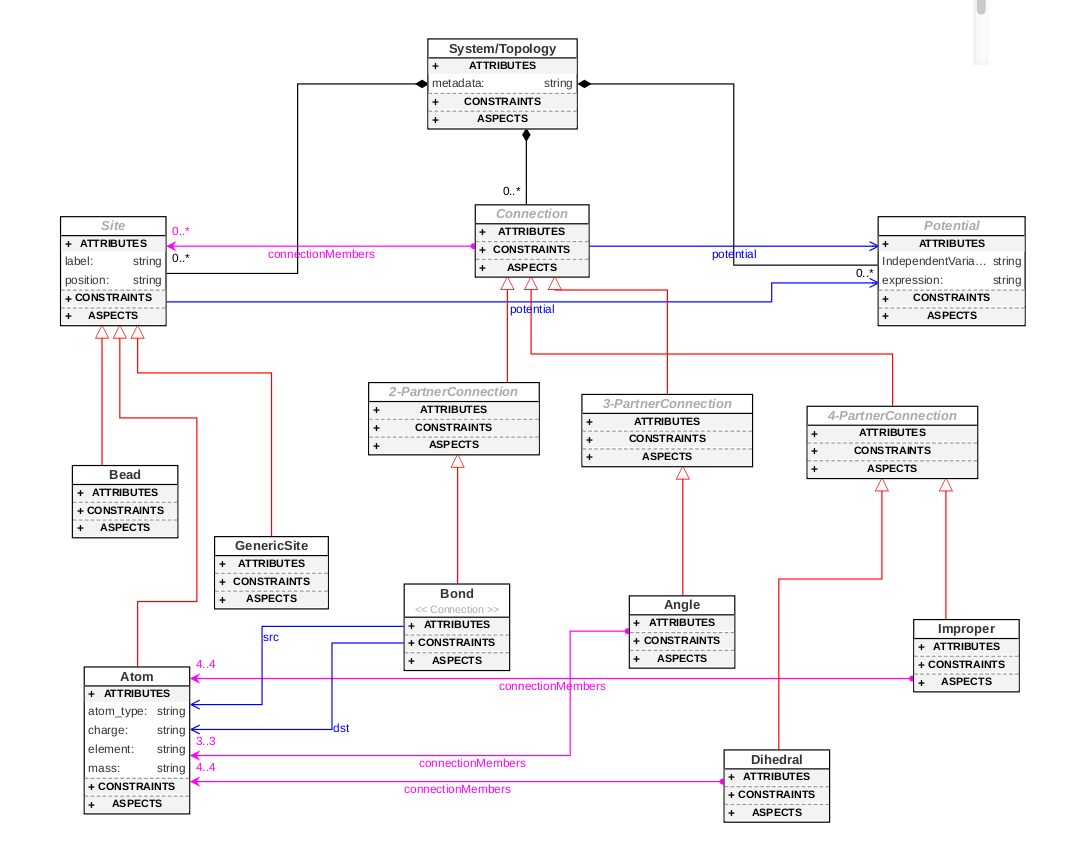
\includegraphics[width=\textwidth]{docs/topo}
    \caption{Overall block diagram of the \texttt{System} container drawn in webgme. Note that (for instance) mass of an \texttt{Atom} is represented as a string signifying the unit system support.}
    \label{fig:TopoDiagram}
\end{figure}

\noindent The overall block diagram of the \texttt{PotentialCollection} container can be represented via webgme meta--model as shown in Figure~\ref{fig:FFDiagram}:

\begin{figure}[ht]
    \centering
    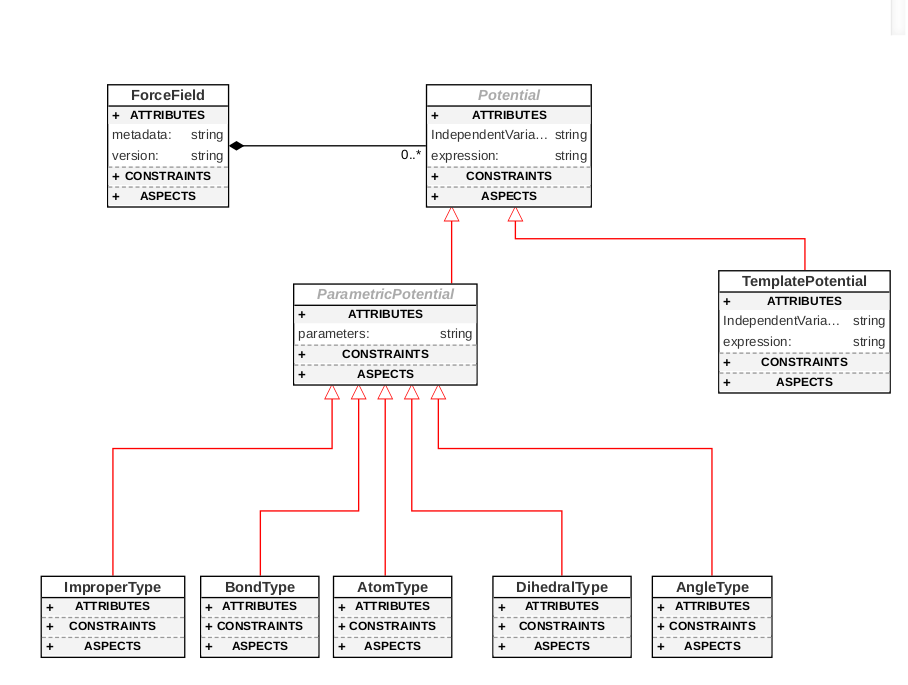
\includegraphics[width=\textwidth]{docs/pot}
    \caption{Overall block diagram of the \texttt{PotentialCollection} container with different \texttt{Potential} variants}
    \label{fig:FFDiagram}
\end{figure}

\section{Next Steps}
While this document provides an introductory specification, it falls short in details and doesn't cover many quirks for this specification to be representative. Next, we plan to investigate non--represented systems as well as further refine the \texttt{PotentialCollection} specification and revise this draft specification for completeness. We also plan to review specification developed by our colleagues at Open--ForceField, determine the shared goals and merge both specifications for a single shared specification.

\section{Conclusion}
This document specified \textbf{GPMSO} specification which can be leveraged to implement extensible base data structures to represent a general purpose molecular simulation object.
\end{document}
